\documentclass[%
 aip,
% jmp,
% bmf,
% sd,
% rsi,
 amsmath,amssymb,
%preprint,%
 reprint,%
%author-year,%
%author-numerical,%
% Conference Proceedings
]{revtex4-1}

\usepackage{graphicx}% Include figure files
\usepackage{dcolumn}% Align table columns on decimal point
\usepackage{bm}% bold math
%\usepackage[mathlines]{lineno}% Enable numbering of text and display math
%\linenumbers\relax % Commence numbering lines

\usepackage[utf8]{inputenc}
\usepackage[T1]{fontenc}
\usepackage{mathptmx}
\usepackage{etoolbox}
\usepackage{hyperref}
\usepackage{float}
\usepackage{svg}

\hypersetup{
    colorlinks=true,
    linkcolor=blue,
    urlcolor=blue,
    linkbordercolor=white
}

%% Apr 2021: AIP requests that the corresponding 
%% email to be moved after the affiliations
\makeatletter
\def\@email#1#2{%
 \endgroup
 \patchcmd{\titleblock@produce}
  {\frontmatter@RRAPformat}
  {\frontmatter@RRAPformat{\produce@RRAP{*#1\href{mailto:#2}{#2}}}\frontmatter@RRAPformat}
  {}{}
}%
\makeatother
\begin{document}

\preprint{AIP/123-QED}

\title[Sample title]{Sample Title:\\with Forced Linebreak}
% Force line breaks with \\
\author{A. Author}
 \altaffiliation[Also at ]{Physics Department, XYZ University.}%Lines break automatically or can be forced with \\
\author{B. Author}%
 \email{Second.Author@institution.edu.}
\affiliation{ 
Authors' institution and/or address%\\This line break forced with \textbackslash\textbackslash
}%

\author{C. Author}
 \homepage{http://www.Second.institution.edu/~Charlie.Author.}
\affiliation{%
Second institution and/or address%\\This line break forced% with \\
}%

\date{\today}% It is always \today, today,
             %  but any date may be explicitly specified

\begin{abstract}
    An article usually includes an abstract, a concise summary of the work
    covered at length in the main body of the article. It is used for
    secondary publications and for information retrieval purposes. 
\end{abstract}

\maketitle

\begin{quotation}
    The ``lead paragraph'' is encapsulated with the \LaTeX\
    %
    The lead paragraph will only be found in an article being prepared for the journal \textit{Chaos}.
\end{quotation}

\section{\label{sec:level1}INTRODUCTION\protect\\ }
% The line break was forced \lowercase{via} \textbackslash\textbackslash
The color of the background represents the order parameter $r$ of the system. The color of the snapshots represents the phase of the oscillators. The color of the arrows represents the direction of the velocity of the oscillators. The size of the arrows represents the speed of the oscillators. 

\section{model}
Oscillators have a spatial position $\mathbf{r}_i=\left( x_i, y_i \right)$ and an internal phase $\theta_i$ which evoleve according to equations:

\begin{eqnarray}
    \dot{x}_i&=&v\cos \theta _i\;,\label{eq:dotxi}
  \\
    \dot{y}_i&=&v\sin \theta _i\;,\label{eq:dotyi}
  \\
    \dot{\theta}_i&=&\omega _i+\lambda \sum_{j=1}^N{A_{ij}\sin \left( \theta _j-\theta _i \right)}
    \label{eq:dotthetai}
\end{eqnarray}
for $i=1,2,\ldots,N$, where $N$ is the number of oscillators. As per Eq.~(\ref{eq:dotxi}) and (\ref{eq:dotyi}), each oscillator moves with a constant speed $v$ in the direction of its current phase $\theta_i$. The phase $\theta_i$ evolves according to Eq.~(\ref{eq:dotthetai}), where $\omega_i$ is the natural frequency of the $i$th oscillator, $\lambda$ is the coupling strength, and $A$ is the adjacency matrix of the network, with $A_{ij}=1$ if there is a connection from $i$th to $j$th oscillator, and $A_{ij}=0$ otherwise. We can consider Eq.~(\ref{eq:dotxi})-(\ref{eq:dotthetai}) as a generalization of the Kuramoto model and the Vicsek model in the sense that it includes both the phase and the spatial position of the oscillators.

Each oscillator $i$ is connected to all the oscillators within a
action radius $d_0$ of its position. The adjacency matrix $A$ is defined as:

\begin{equation}
    A_{ij}=\begin{cases}
        1,&		\left| \mathbf{r}_i-\mathbf{r}_j \right|\le d_0\\
        0,&		\left| \mathbf{r}_i-\mathbf{r}_j \right|>d_0\\
    \end{cases}
\end{equation}
where $\left| \mathbf{r}_i-\mathbf{r}_j \right|$ is the Euclidean distance between the $i$th and $j$th oscillators. 

For simplicity, we consider oscillators are initially distributed uniformly in a two-dimensional square with side length $L$ and periodic boundary conditions. Their positions $\mathbf{r}_i\left( t \right) =\left( x_i\left( t \right) ,y_i\left( t \right) \right) $ at given time $t$ are given by:

\begin{equation}
    \begin{array}{c}
        x_i\left( t+\Delta t \right) =x_i\left( t \right) +v\cos \theta _i\left( t \right) \Delta t\,\,\mathrm{mod}\ L,\\
        x_i\left( t+\Delta t \right) =x_i\left( t \right) +v\cos \theta _i\left( t \right) \Delta t\,\,\mathrm{mod}\ L,\\
    \end{array}
\end{equation}
where $\Delta t$ is the discrete time step. When two oscillators are on opposite sides of the square, the absolute value of the difference between one of their coordinates is greater than $L/2$. In this case, we take the minimum distance between them, which is the distance between the two points in the periodic boundary conditions. For a given pair of points $\mathbf{r}_i$ and $\mathbf{r}_j$, the distance between them is $\left| \mathbf{r}_i-\bar{\mathbf{r}}_j \right|$, where $\bar{\mathbf{r}}_j=\left( \bar{x}_j,\bar{y}_j \right)$ is the adjusted position of the $j$th oscillator, given by:
\begin{eqnarray}\label{eq:adj_pos1}
    \bar{x}_j=\begin{cases}
        x_j,&		\left| x_i-x_j \right|\le L/2\\
        x_j+L,&		x_i-x_j>L/2\\
        x_j-L,&		x_i-x_j>L/2\\
    \end{cases},
    \\
    \bar{y}_j=\begin{cases}\label{eq:adj_pos2}
        y_j,&		\left| y_i-y_j \right|\le L/2\\
        y_j+L,&		y_i-y_j>L/2\\
        y_j-L,&		y_i-y_j>L/2\\
    \end{cases}.
\end{eqnarray}
$\left| \mathbf{r}_i-\bar{\mathbf{r}}_j \right|$ can be proved to be the minimum distance between $\mathbf{r}_i$ and $\mathbf{r}_j$ in the periodic boundary conditions (see the proof in Appendix \ref{sec:adj_pos}).

Finally, we consider that the natural frequencies $\omega_i$ are distributed in two symmetric uniform distributions. Exactly half of the oscillators have natural frequencies in the range $\left[ \omega _{\min},\omega _{\max} \right]$ ($\omega_i \sim U\left( \omega _{\min},\omega _{\max} \right), i=1,2,\ldots,N/2$) and the other half in the range $\left[ -\omega _{\max},-\omega _{\min} \right]$ ($\omega_i \sim U\left( -\omega _{\max},-\omega _{\min} \right), i=N/2+1,N/2+2,\ldots,N$).

\section{behavior}

\begin{figure*}
    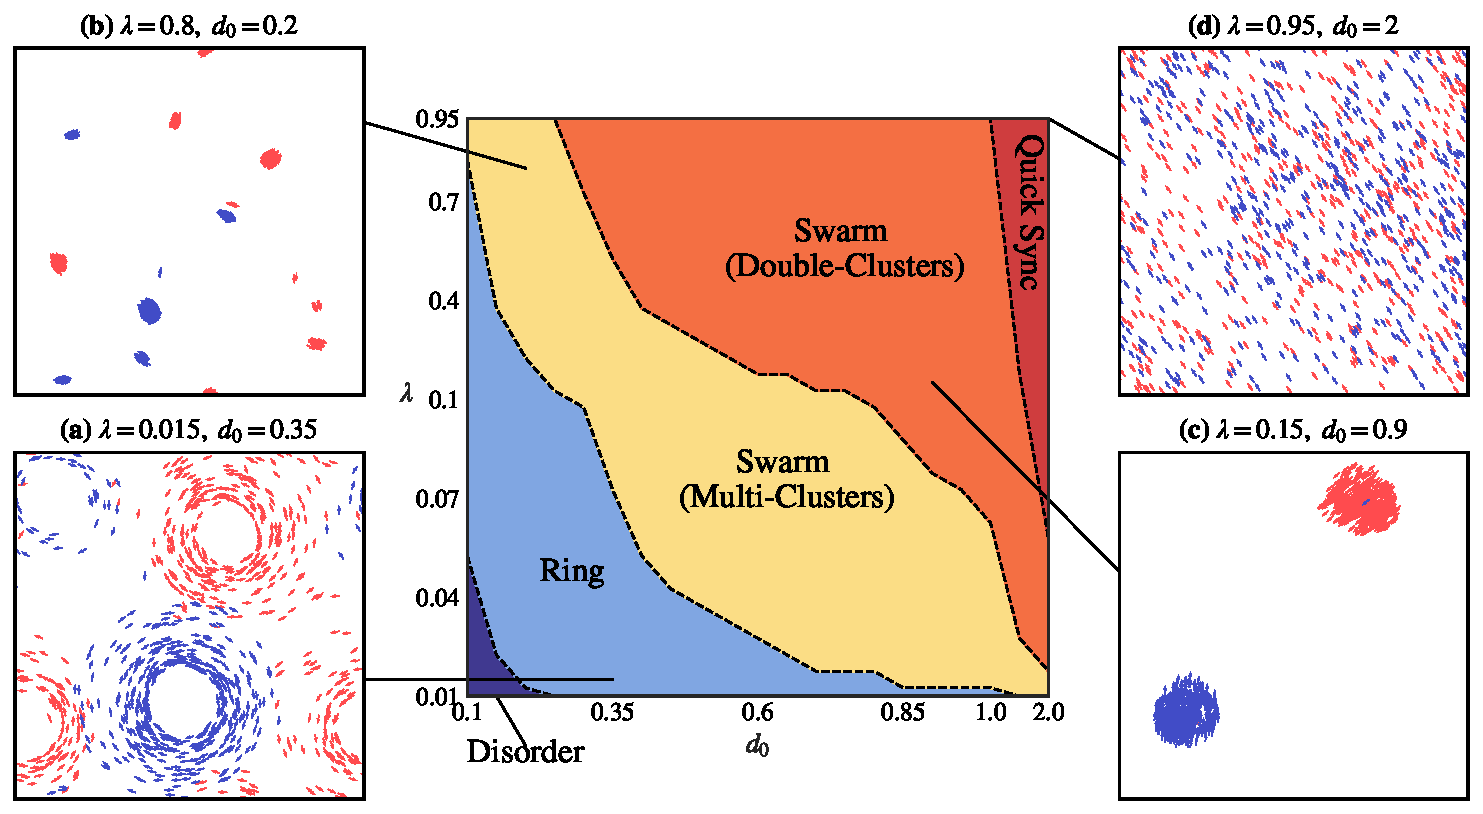
\includegraphics[width=\textwidth]{./figs/phaseDiagram.pdf}
    \caption{
        \label{fig:phaseDiagram} Phase diagram of model Eq.~(\ref{eq:dotxi})-(\ref{eq:dotthetai}) in the $(\lambda$-$d_0)$ plane. The boundaries between states is 
        analytical approximations given by Section~\ref{analytical}. 
        For the sake of clarity, the scale of $\lambda$ and $d_0$ is non-linear (For $\lambda$ in $\left[ 0.01, 0.1 \right]$ and $\left[ 0.1, 1 \right]$, step length is $0.1$ and $0.05$, respectively. For $d_0$ in $\left[ 0.1, 1 \right]$ and $\left[ 1, 2 \right]$, step length is $0.05$ and $0.5$, respectively).
        \textbf{(a)}, The snapshots of Ring ($\lambda=0.015,\ d_0=0.35$). 
        \textbf{(b)}, Swarm (Multi-Clusters) ($\lambda=0.8,\ d_0=0.2$).
        \textbf{(c)}, Swarm (Double-Clusters) ($\lambda=0.15,\ d_0=0.9$).
        \textbf{(d)}, Quick Sync ($\lambda=0.95,\ d_0=2$). Two types of chiral oscillators are represented by red ($\omega_i > 0$) and blue 
        ($\omega_i < 0$) arrows, respectively. 
    }
\end{figure*}

\begin{figure}[b]
    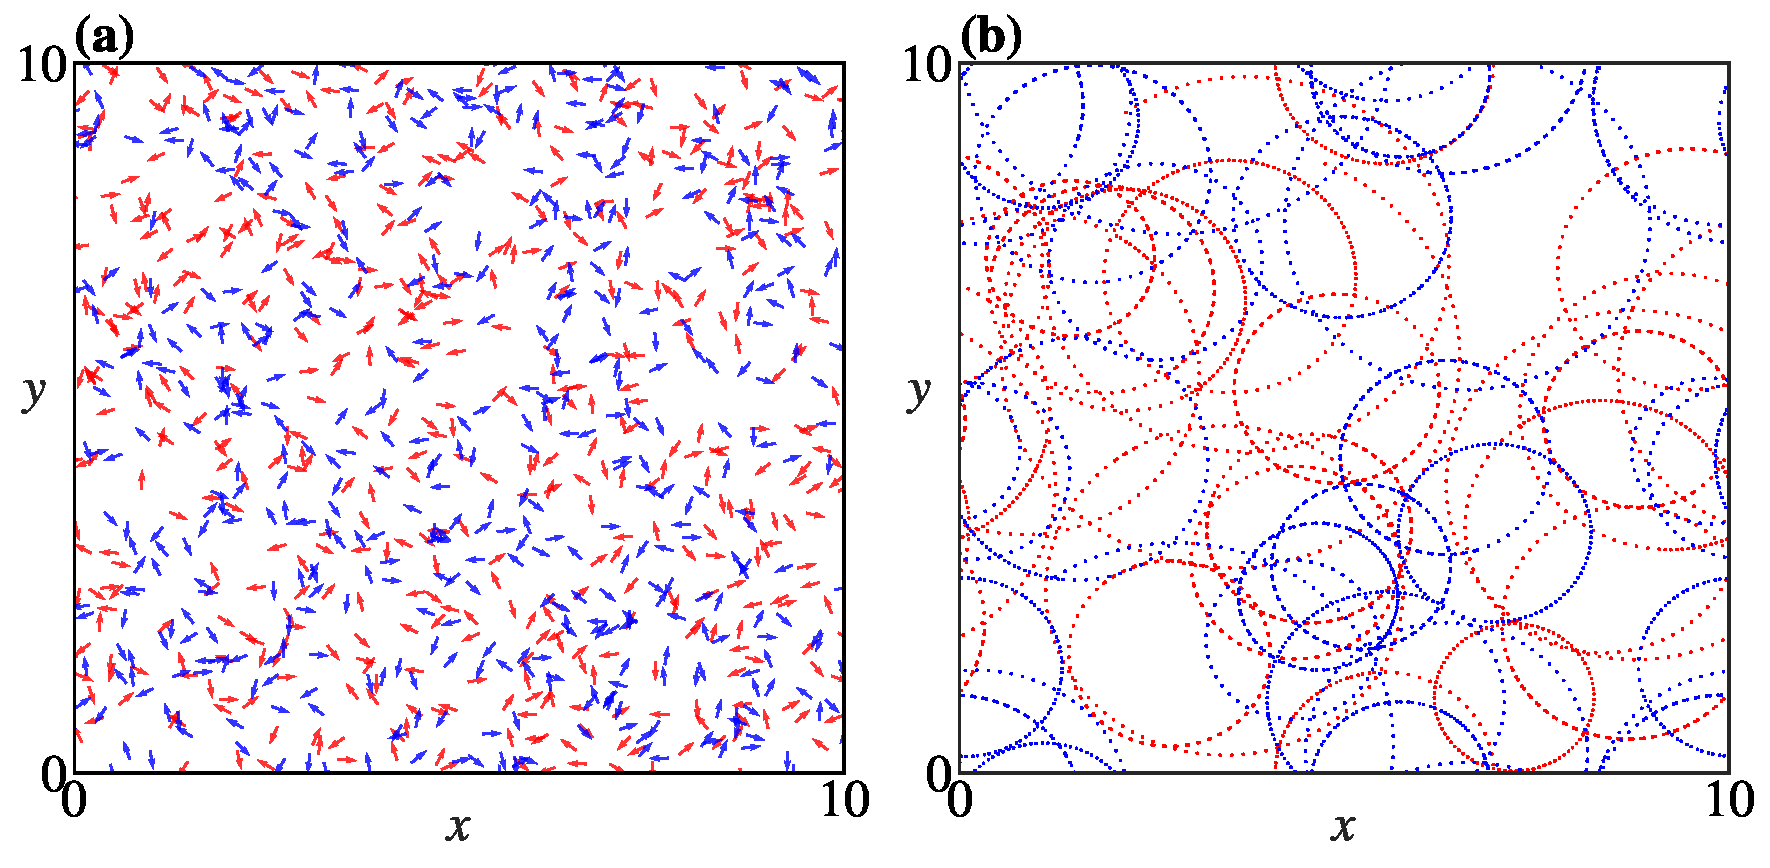
\includegraphics[width=0.48\textwidth]{./figs/disorderState.pdf}
    \caption{
        \label{fig:disorderState} Key properties of the Disorder state. 
        \textbf{(a)}, The snapshot of the Disorder state ($\lambda=0.01,\ d_0=0.1, T=60000$). 
        \textbf{(b)}, The scatter plot of last 100 time steps of 20 positive chirality oscillators and 20 negative chirality oscillators.
    }
\end{figure}

We performed numerical simulations of the model to probe the behavior of its solutions (see Appendix \ref{sec:numerics} for details on the numerical methods). 
$N=1000$ oscillators were distributed uniformly in the square of length $L=10$ and their natural frequencies were distributed in the range $\left[ \omega _{\min},\omega _{\max} \right]=\left[ 1,3 \right]$ and $\left[ -\omega _{\max},-\omega _{\min} \right]=\left[ -3,-1 \right]$.
Two-parameter of coupling strength $\lambda$ and action radius $d_0$ are presented in the phase diagram in Fig.~\ref{fig:phaseDiagram}. We found the system settles into five states: \textbf{Disorder}, \textbf{Ring}, \textbf{Swarm} (which can be further divided into \textbf{Multi-Clusters} and \textbf{Double-Clusters}), and \textbf{Quick Sync}. In Fig.~\ref{fig:phaseDiagram} we show the snapshots of the last three states and where these states are located in the phase diagram. The Disorder state is shown in Fig.~\ref{fig:disorderState}a.
We next discuss these five states.

\begin{figure*}
    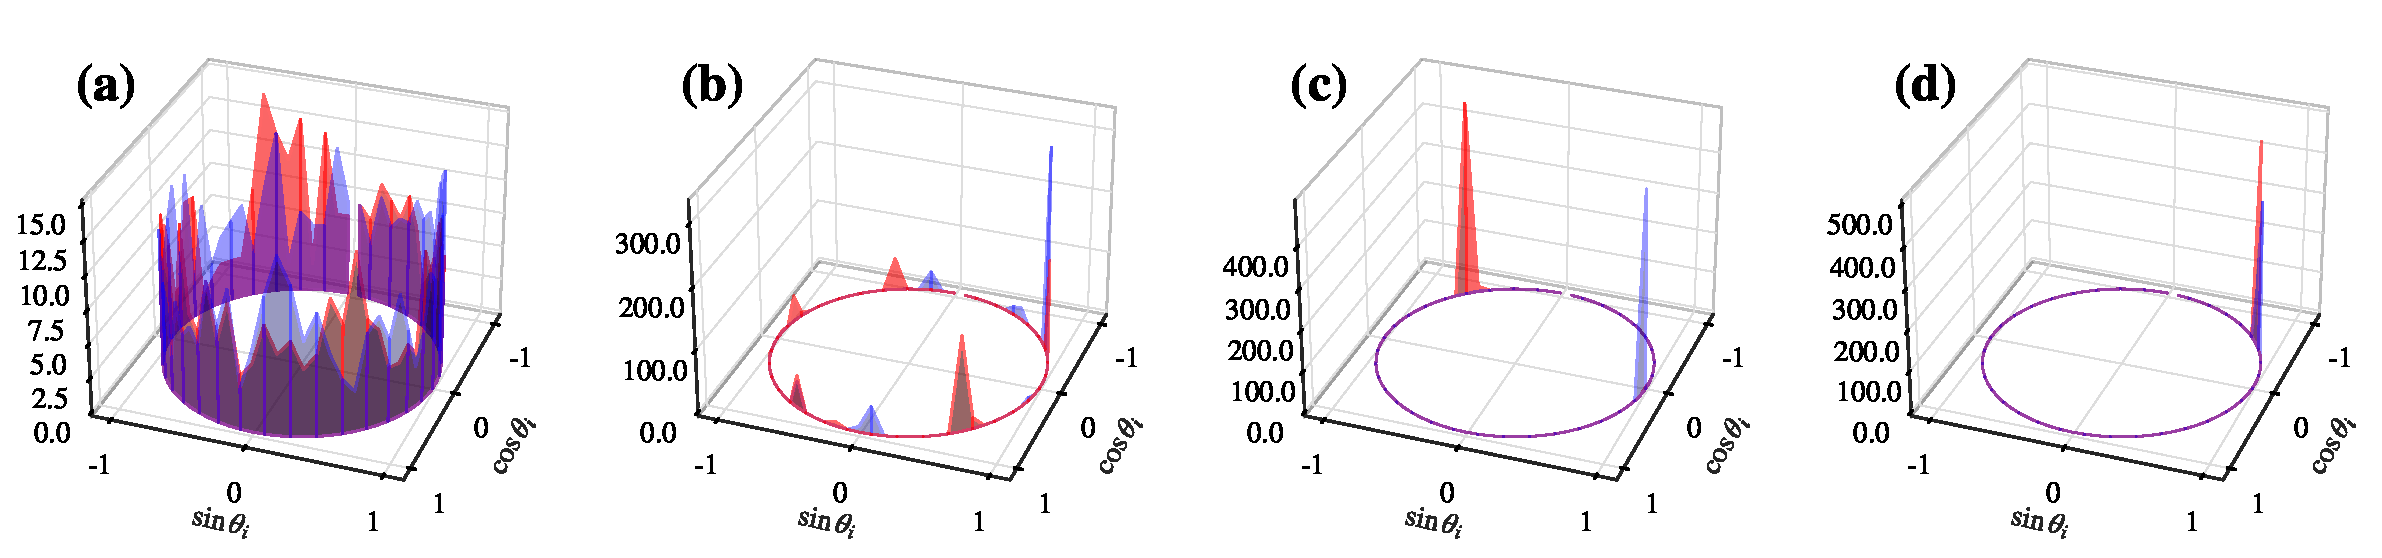
\includegraphics[width=\textwidth]{./figs/phaseHist.pdf}
    \caption{
        \label{fig:phaseHist} Histogram of the oscillators' phases.
        \textbf{(a)}, Ring state ($\lambda=0.015,\ d_0=0.35$).
        \textbf{(b)}, Swarm state (Multi-Clusters, $\lambda=0.8,\ d_0=0.2$).
        \textbf{(c)}, Swarm state (Double-Clusters, $\lambda=0.15,\ d_0=0.9$).
        \textbf{(d)}, Quick Sync state ($\lambda=0.95,\ d_0=2$). The histograms are calculated with $70$ bins.
    }
\end{figure*}



\subsection{Disorder State}

Disorder state occurs when both $\lambda$ and $d_0$ are small. In this state, the oscillators are not asynchronous (phase histogram is uniform, like Fig.~\ref{fig:phaseHist}a) and move in a way which similar to uncoupled oscillators ($\lambda=0$), as shown in Fig.~\ref{fig:disorderState}a. According to Eq.~(\ref{eq:dotxi})-(\ref{eq:dotthetai}), when $\lambda=0$, the equations of oscillators' motion can be written as:

\begin{equation}
    \begin{array}{c}
        x_i\left( t \right) =x_i\left( 0 \right) +\frac{v}{\omega _i}\sin \omega _it\;,\\
        y_i\left( t \right) =y_i\left( 0 \right) +\frac{v}{\omega _i}\cos \omega _it\;.\\
    \end{array}
\end{equation}
In such a setup, oscillators move in a circular trajectory with radius $v/\omega _i$ and the phases $\theta_i$ increase linearly with time, as show in Fig.~\ref{fig:disorderState}b. To calculate the real-time rotational radius, we first estimate real-time centers $\mathbf{c}(t)$ of the circular trajectory with method in Fig.~\ref{fig:CenterEps} and then solve the following linear equations:

\begin{figure}[b]
    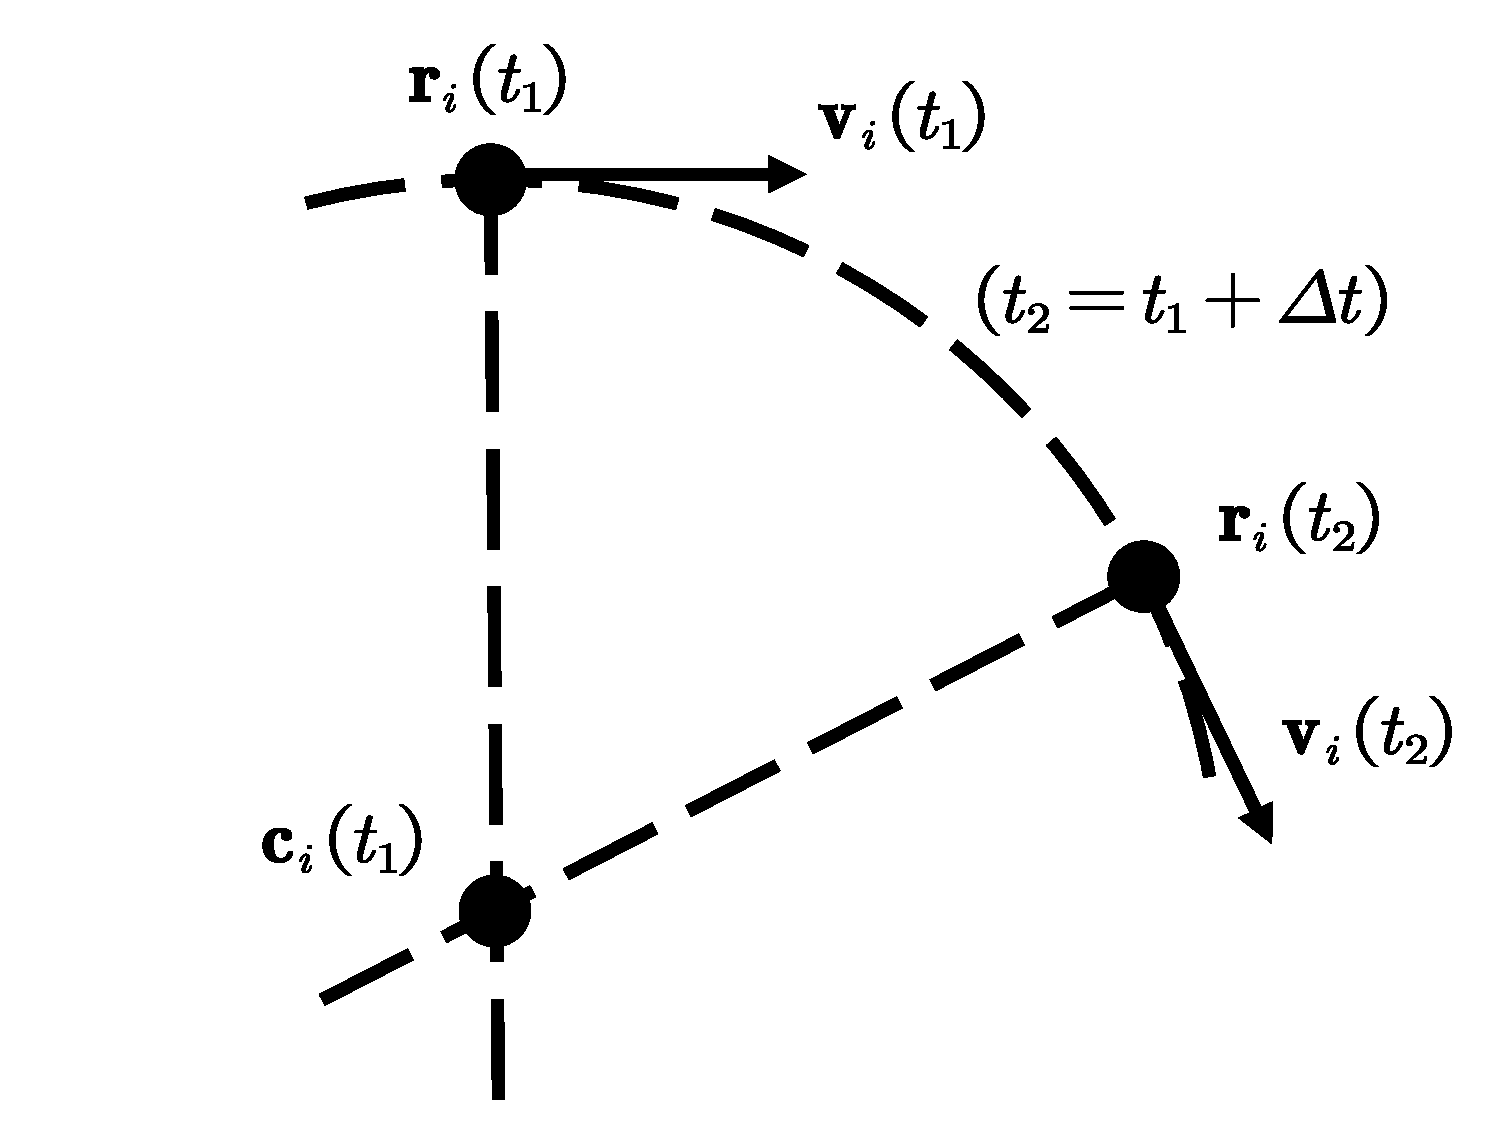
\includegraphics[width=0.25\textwidth]{./figs/CenterEps.pdf}
    \caption{\label{fig:CenterEps} Estimation for real-time centers. $\mathbf{v}_i(t_1)$ and $\mathbf{r}_i(t_1)$ are the velocity and position of $i$th oscillator at $t_1$, respectively. According to Eq.~(\ref{eq:dotxi})-(\ref{eq:dotthetai}), we can calculate $\mathbf{v}_i(t_2)$ and $\mathbf{r}_i(t_2)$, ($t_2=t_1+\Delta t$). 
    The line $\mathbf{c}_i(t)\mathbf{v}_i(t)$ is perpendicular to $\mathbf{v}_i(t)$.}
\end{figure}

\begin{equation}\label{eq:linearEquations}
    \begin{array}{c}
        \mathbf{c}_i\left( t_1 \right) \cdot \mathbf{v}_i\left( t_1 \right) =\mathbf{x}_i\left( t_1 \right) \cdot \mathbf{v}_i\left( t_1 \right)\;,\\
        \mathbf{c}_i\left( t_2 \right) \cdot \mathbf{v}_i\left( t_2 \right) =\mathbf{x}_i\left( t_2 \right) \cdot \mathbf{v}_i\left( t_2 \right)\;.\\
    \end{array}
\end{equation}
 
\begin{figure*}
    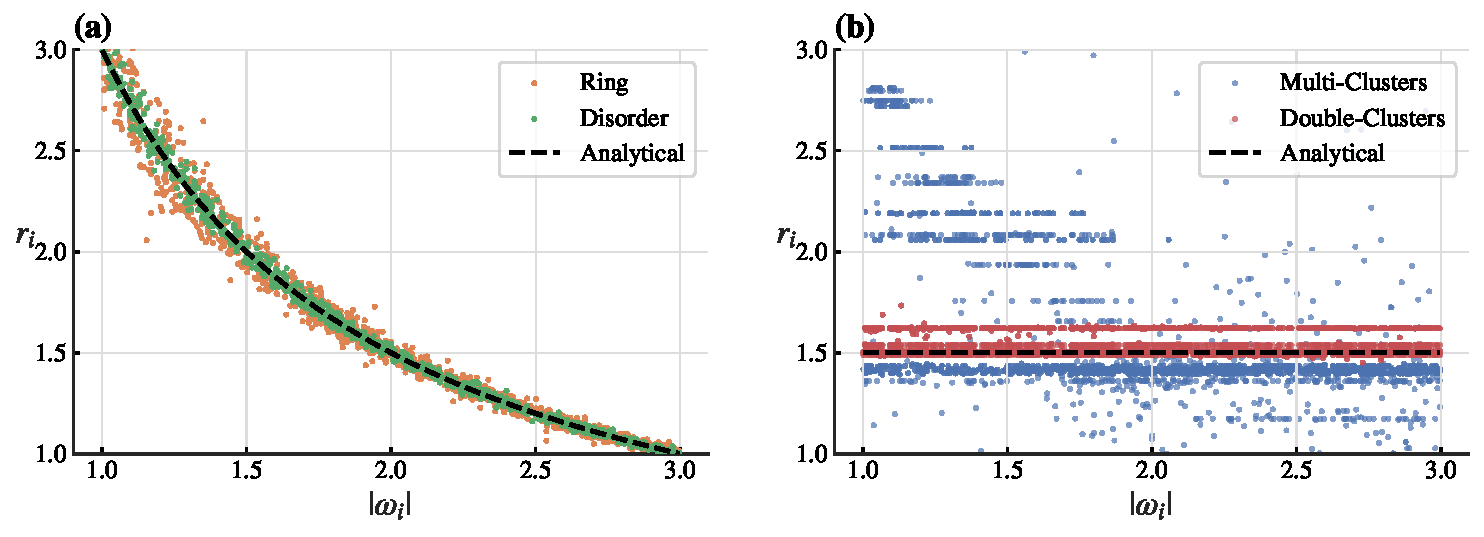
\includegraphics[width=\textwidth]{./figs/radiusOmega.pdf}
    \caption{
        \label{fig:radiusOmega} The real-time and analytical rotational radius.
        \textbf{(a)}, Radius for the Disorder ($d_0=0.1$, $\lambda=0.01:0.06$) and Ring ($d_0=0.1$, $\lambda=0.06:0.1$). The real-time rotational radius is almost constant and close to $v/\omega_i$ for each oscillator. 
        \textbf{(b)}, Radius for Swarm (Multi-Clusters, $d_0=0.15:0.25$, $\lambda=0.95$) and (Double-Clusters, $d_0=2$, $\lambda=0.02:0.05$). Line of Analytical is only for Double-Clusters.
        All the above simulations are calculated at $t=60000$. 
    }
\end{figure*}

The real-time rotational radius is $r_i(t)=\left| \mathbf{c}_i(t)-\mathbf{r}_i(t) \right|$. We found that the real-time rotational radius is almost constant and close to $v/\omega_i$ for each oscillator in the Disorder state, as shown in Fig.~\ref{fig:radiusOmega}a.

\begin{figure*}
    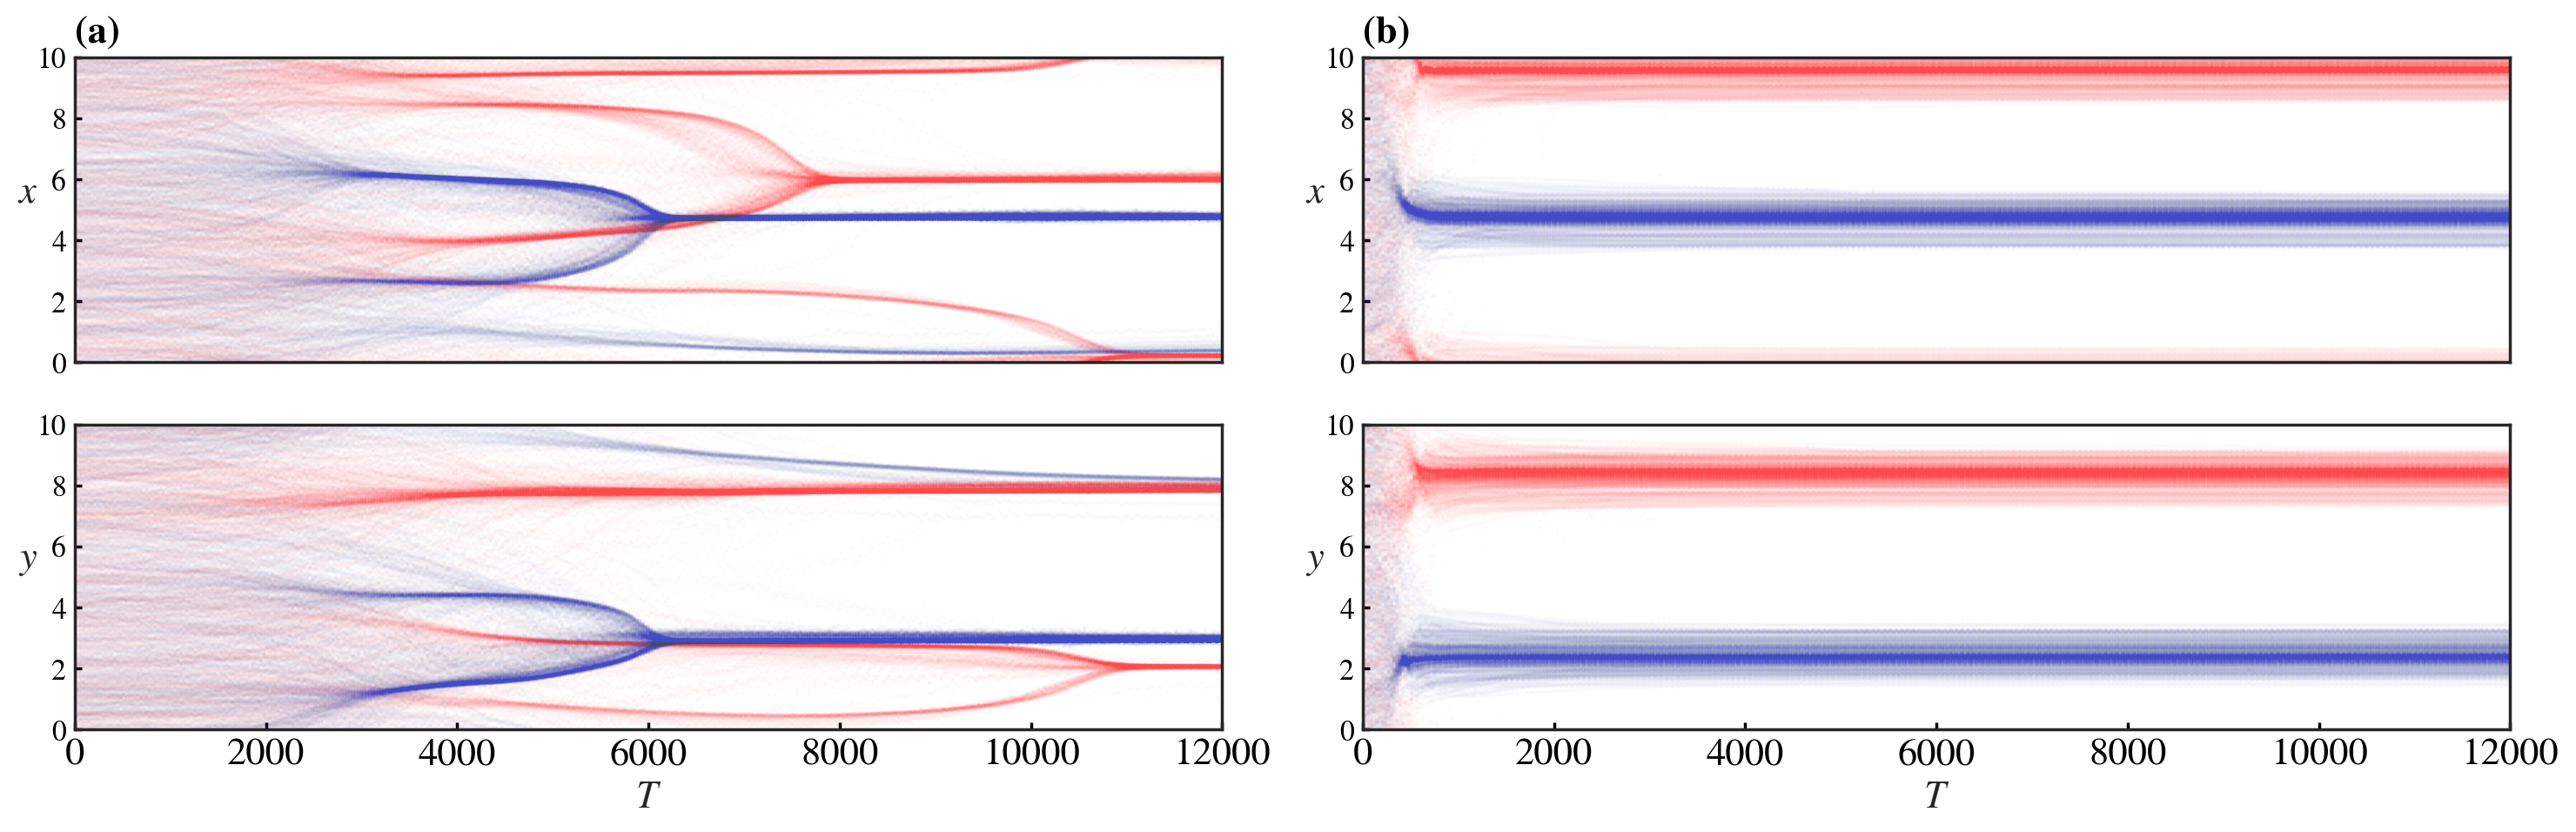
\includegraphics[width=\textwidth]{./figs/centersPosition.png}
    \caption{
        \label{fig:centersPosition} Scatter plot of the real-time centers position. 
        \textbf{(a)}, centers position of Ring ($\lambda=0.02$, $d_0=0.4$). As time goes on, the centers of oscillators with the same chirality converge.
        \textbf{(b)}, centers position of Swarm ($\lambda=0.01$, $d_0=2$). Unlike Ring, the centers converge quickly.
        The centers position are estimated with method in Fig.~\ref{fig:CenterEps} and Eq.~(\ref{eq:linearEquations}).
    }
\end{figure*}

\begin{figure}[b!]
    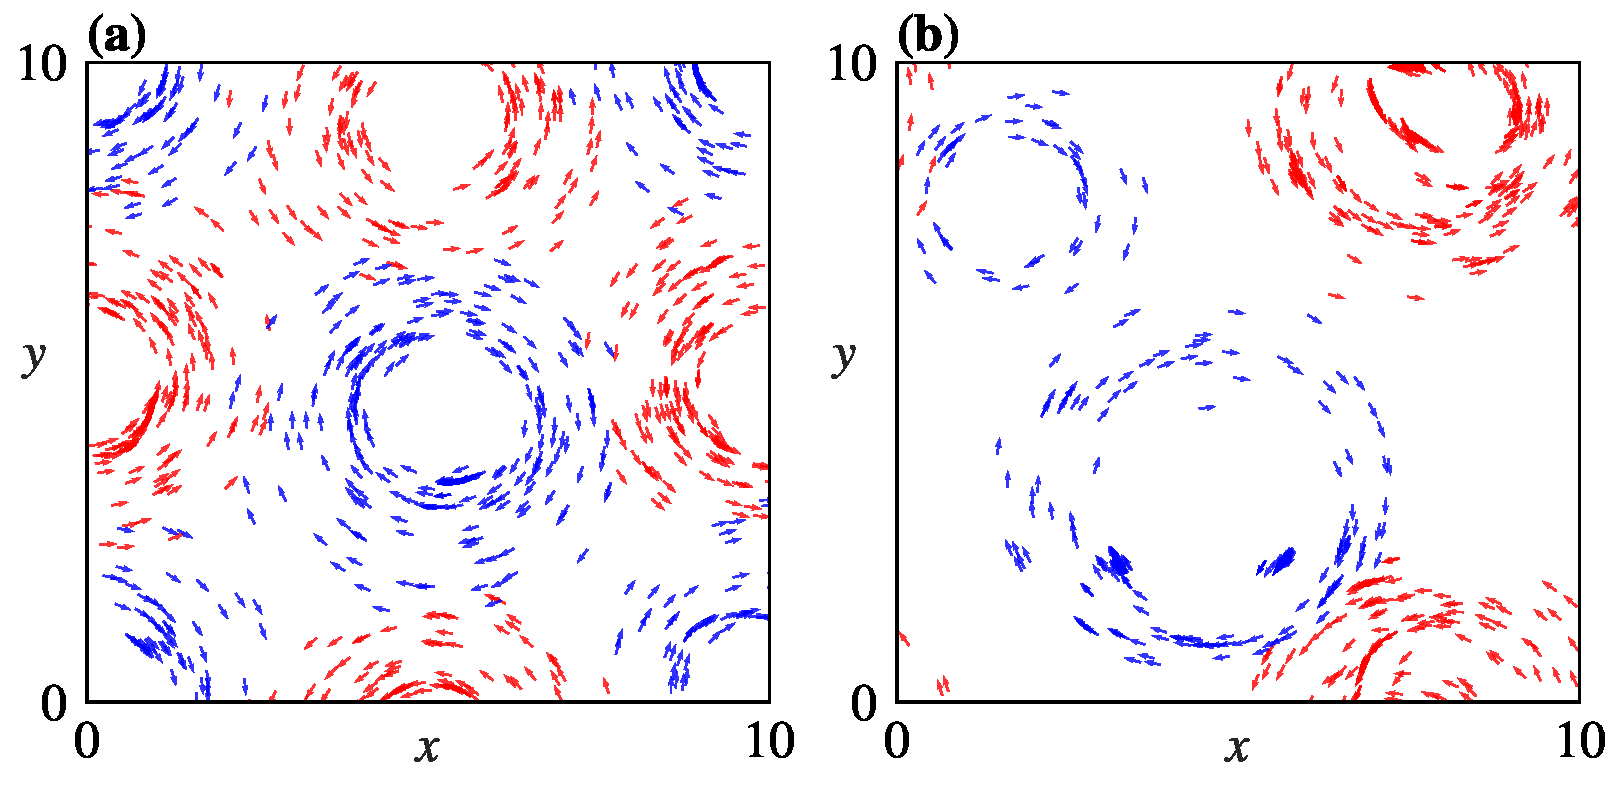
\includegraphics[width=0.48\textwidth]{./figs/ringStateNum.pdf}
    \caption{
        \label{fig:ringStateNum} Snapshots of the Ring state. 
        \textbf{(a)}, Four rings ($\lambda=0.02$, $d_0=0.4$). 
        \textbf{(b)}, Three rings ($\lambda=0.025$, $d_0=0.45$).
    }
\end{figure}

\subsection{Ring State}

The Ring state is characterized by the oscillators forming several rings with thickness, each of which is composed of oscillators with the same chirality, as is show in Fig.~\ref{fig:phaseDiagram}a. 
Similar to Disorder state, the oscillators in the same ring cluster move in a circular trajectory with a constant rotational radius calculated in Fig.~\ref{fig:radiusOmega}a. 
The oscillators' phase is uniformly distributed in the range $\left[ -\pi,\pi \right]$ (cf. Fig.~\ref{fig:phaseHist}a), which leads to oscillators uniformly located on the circular trajectory.
Fig.~\ref{fig:centersPosition}a shows there is a long transient time before this state is reached, and in this transient time, the trajectories of oscillators with the same chirality aggregate slowly. Conversely, the oscillators with different chirality repel each other. 
For parameter plane in Fig.~\ref{fig:phaseDiagram}, the number of ring decreases and local swarms appear at high-frequency ($\left|\omega_i\right|\rightarrow \omega_{\max}$) oscillators with $\lambda$ and $d_0$ increasing, as is shown in Fig.~\ref{fig:ringStateNum}a. 


\subsection{Swarm State}

Swarm State is a state where the oscillators form spatial clusters and align into several clusters [Fig.~\ref{fig:phaseDiagram}b, c and Fig.~\ref{fig:centersPosition}b]. When $\lambda$ and $d_0$ increases, the number of clusters decreases by 2, which is named by as Double-Clusters state, and other states are named by Multi-Clusters state. The clusters are composed of oscillators with the same chirality, and the phase $\theta_i$ of the oscillators in the same cluster is synchronized as seen in Fig.~\ref{fig:phaseHist}b and \ref{fig:phaseHist}c, which means that the oscillators in the cluster move with the same velocity $\mathbf{v}_i=\left( \cos \theta _s,\ \sin \theta _s \right)$ and rotational radius $r_i=v/\theta_s$, where $\theta_s$ is the oscillators' phase in the cluster. Based on this property, we can calculate $\theta_s$ and $r_i$ with Eq.~(\ref{eq:dotthetai}):

\begin{equation}\label{eq:clusterState}
    \begin{aligned}
        N_s\omega _s&=\sum_{i=1}^{N_s}{\left( \omega _i+\lambda \sum_{j=1}^{N_s}{A_{ij}\sin \left( \theta _j-\theta _i \right)} \right)}\\
        \omega _s&=\frac{1}{N_s}\sum_{i=1}^{N_s}{\omega _i}+\frac{\lambda}{N_s}\sum_{i=1}^{N_s}{\sum_{j=1}^{N_s}{A_{ij}\sin \left( \theta _j-\theta _i \right)}}\\
        &=\frac{1}{N_s}\sum_{i=1}^{N_s}{\omega _i}\;,\\
    \end{aligned}
\end{equation}
where $N_s$ is the number of oscillators in the cluster.
As $\omega_i \sim U\left( \omega _{\min},\omega _{\max} \right)$ and $\omega_i \sim U\left( -\omega _{\max},-\omega _{\min} \right)$ for two types of chirality, we can calculate $\theta_i$, $\omega_s$ and $r_i$ with $\omega_i$ for Double-Clusters state:

\begin{equation}
    \begin{aligned}
        \theta _i&=\omega _s=\begin{cases}
        \left( \omega _{\max}+\omega _{\min} \right) /2,&		i=1,2,\dots ,N/2\\
        -\left( \omega _{\max}+\omega _{\min} \right) /2,&		i=N/2+1,\cdots ,N\\
    \end{cases}\,\,,\\
        r_i&=\frac{v}{\omega _s}\;,\\
    \end{aligned}
\end{equation}
as shown in Fig.~\ref{fig:radiusOmega}b. But for Multi-Clusters, due to which oscillators are synchronized within each cluster is not accurately known, we can only calculate the real-time rotational radius of the them. As seen in Fig.~\ref{fig:radiusOmega}b, similar to Double-Clusters, some local platforms appear in the real-time rotational radius due to synchronization.

\subsection{Quick Sync State}

Quick Sync state is a simple state where total oscillators are synchronized quickly, as shown in Fig.~\ref{fig:phaseDiagram}d. and \ref{fig:phaseHist}d. The oscillators are synchronized in an extremely short time, which leads them have no time to form clusters (can also be considered as a special case of Swarm state). Due to the two types of chirality oscillators are synchronized and the distributions of them is symmetric, the phase velocities of total oscillators are close to zero according to Eq.~(\ref{eq:clusterState}).

\begin{figure*}
    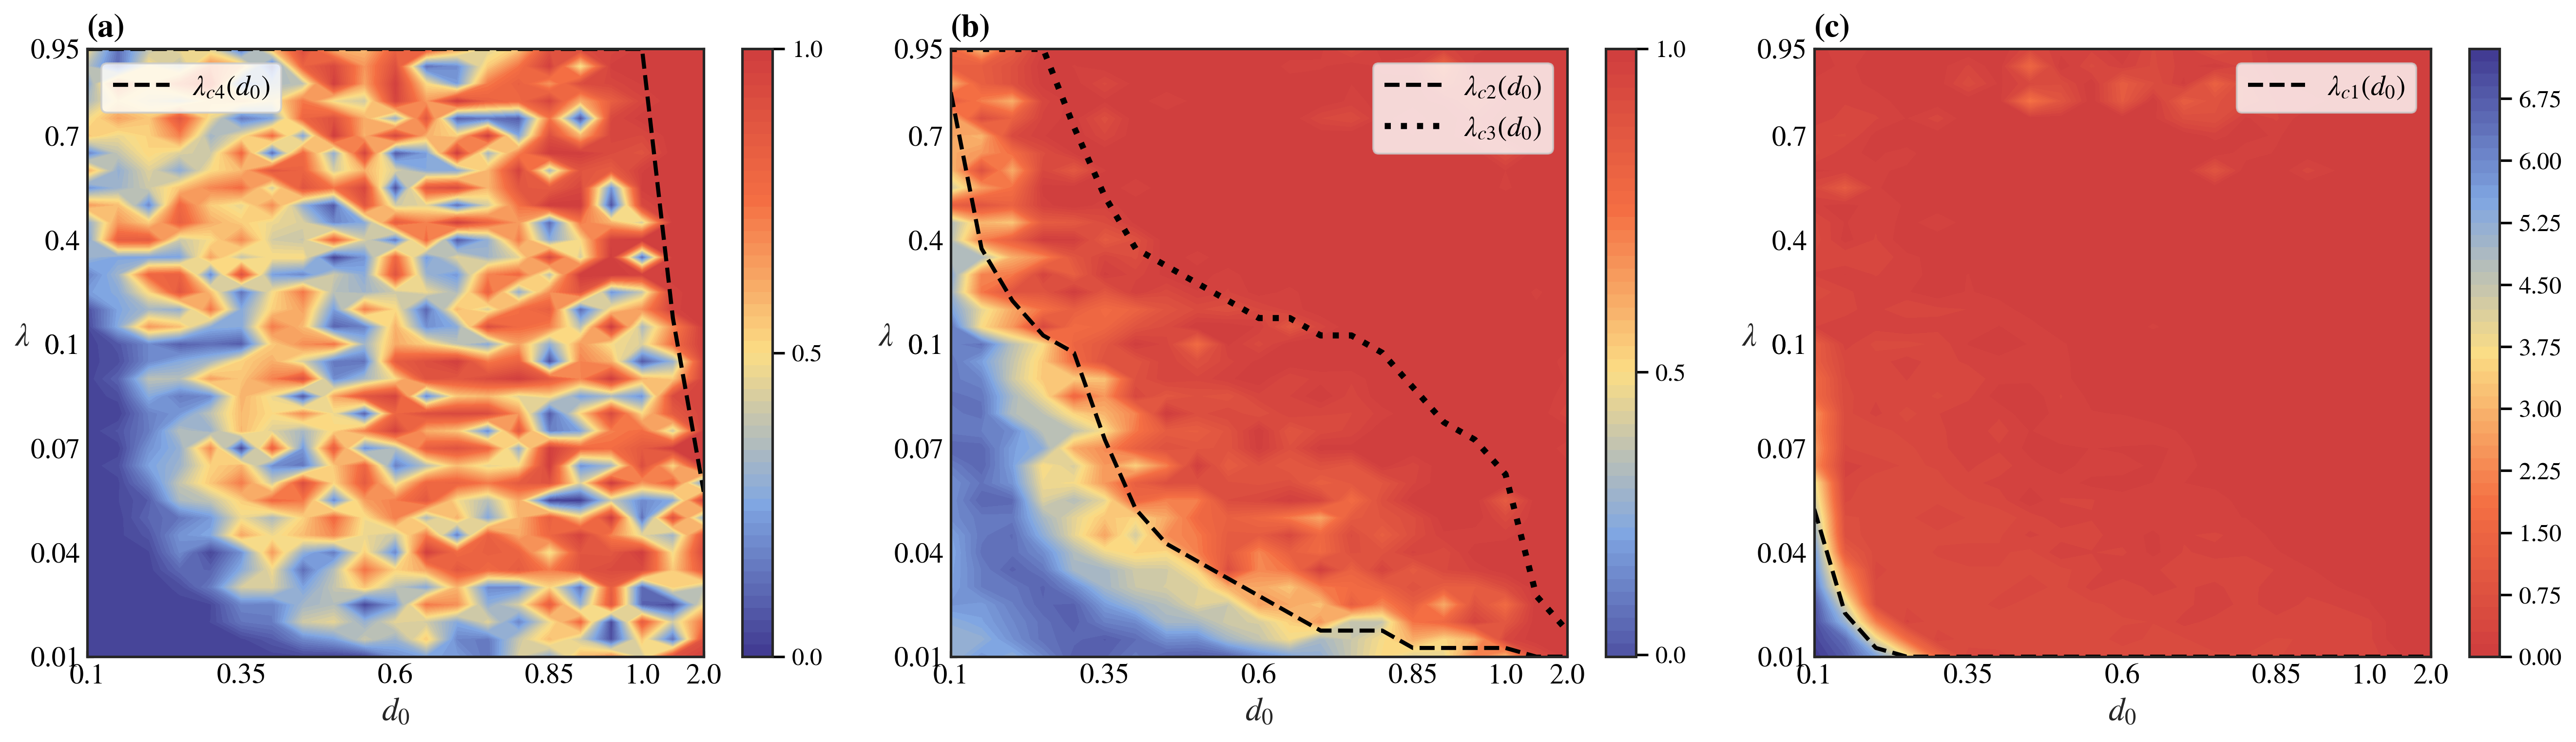
\includegraphics[width=\textwidth]{./figs/orderParam.png}
    \caption{
        \label{fig:orderParam} Order parameter heatmaps of ($\lambda$, $d_0$) plane. 
        \textbf{(a)}, order parameter $R$ and critical line of $\lambda_{c4}$.
        \textbf{(b)}, order parameter $R_s$ and critical lines of $\lambda_{c2}$, $\lambda_{c3}$.
        All order parameters are calculated at $t=60000$
    }
\end{figure*}

\section{Order Parameter}

Having described the four states of our system, we next discuss how to distinguish them. We use the order parameter $R$ to metric global synchronization. The order parameter $R$ is defined as:

\begin{equation}
    R=\left| \frac{1}{N}\sum_{j=1}^N{e^{i\theta _j}} \right|\;.
\end{equation}
The order parameter $R$ is absolute value of the mean of the complex numbers $e^{i\theta _i}$, which can be interpreted as the mean direction of the oscillators.
When $R=1$, the oscillators are completely synchronized, and when $R=0$, the oscillators are completely desynchronized. Fig \ref{fig:orderParam}a shows the order parameter $R$ in the parameter plane. The order parameter $R$ is close to $1$ in the Quick Sync state, close to $0$ in the Disorder state and most of the Ring state, and between $0$ and $1$ in other states. In these states, We see the order parameter $R$ changes non-monotonically in the sense that phases in these states are not globally synchronized and each cluster's phase velocity $\omega_s\ne 0$. When the phases of different clusters are exactly equal, the order parameter $R$ is close to $1$, and when they are exactly opposite, $R$ is close to $0$. 

Having realized that the order parameter $R$ is not enough to distinguish the states with clusters, we next define the following order parameter $R_s$ to metric the local synchronization,

\begin{equation}
    R_s=\frac{1}{N_s}\sum_{k=1}^{N_s}{\left| \frac{1}{\left| C_k \right|}\sum_{j\in C_k}{e^{i\theta _j}} \right|}\;,
\end{equation}
where $N_s$ is the number of clusters, $C_k$ is the $k$th cluster, and $\left| C_k \right|$ is the number of oscillators in the $k$th cluster. We can consider $R_s$ as an order parameter that studies the spatial position and internal phase simultaneously.
To estimate the number of clusters, we use the following method: we first calculate the relative center distance matrix $D_{ij}=\left| \mathbf{c}_i-\bar{\mathbf{c}}_j \right|$, where $\bar{\mathbf{c}}_j=
\left( \bar{x}_j,\bar{y}_j \right)$ is the adjusted position of the $j$th oscillator's rotational center calculated by Eq.~(\ref{eq:adj_pos1}), (\ref{eq:adj_pos2}) and (\ref{eq:linearEquations}). Then we use the DBSCAN algorithm to cluster the oscillators. The DBSCAN algorithm is a density-based clustering algorithm, which can find clusters of arbitrary shapes and sizes. We set the minimum number of oscillators in a cluster to be $10$ and the maximum distance between two oscillators in the same cluster to be $0.3$ (see Appendix \ref{sec:DBSCAN_param} for details on the determination of these parameters). We then calculate the order parameter $R_s$ for each cluster. The order parameter $R_s$ is close to $1$ in the Swarm state and Quick Sync state, and close to $0$ in Disorder state and most of the Ring state, between $0$ and $1$ in other Ring states with local clusters, as shown in Fig.~\ref{fig:orderParam}b.

Combining the order parameter $R$ and $R_s$, we can find only the distinction between Ring and Disorder states has not been resolved. 

\section{\label{analytical} analytical approximations}

\section{CONCLUSIONS}

\appendix

\section{\label{sec:adj_pos} PROOF OF THE ADJUSTED POSITION}


\section{\label{sec:numerics} NUMERICAL METHODS}

All the simulations of the model Eq.~(\ref{eq:dotxi})-(\ref{eq:dotthetai}) were run on Python using Euler integration, with a time step $\Delta t=0.01$, and a total time of $T=60000$. 

\section{\label{sec:DBSCAN_param} Determination of DBSCAN's parameters}

DBSCAN (Density-Based Spatial Clustering of Applications with Noise) is a density-based clustering algorithm, which can find clusters of arbitrary shapes and sizes. The algorithm has two parameters: $\varepsilon$ and $m$. $\varepsilon$ is the maximum distance between two samples for one to be considered as in the neighborhood of the other, and $m$ is the minimum number of samples in a neighborhood for a point to be considered as a core point. 

We set the minimum number of oscillators in a cluster to be $10$ and the maximum distance between two oscillators in the same cluster to be $0.3$. We determined these parameters as follows. 
We traverse all values between $0.1$ and $0.5$ with a step length of $0.1$, and for each value of $\varepsilon$, we calculate the number of clusters with $m=0$.

\begin{figure}[H]
    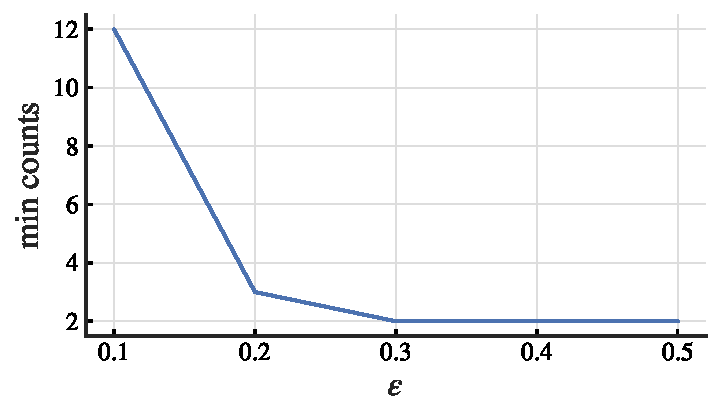
\includegraphics[width=0.48\textwidth]{./figs/DBSCANparam.pdf}
    \caption{
        \label{fig:DBSCANparam} The number of clusters with different $\varepsilon$, $m=0$. The number of clusters is calculated with the DBSCAN algorithm. 
    }
\end{figure}
As shown in Fig.~\ref{fig:DBSCANparam}, the minimum counts of clusters $2$ (corresponding to Double-Clusters state of Swarm) first appear at $\varepsilon=0.3$. Then we set $\varepsilon$ to be $0.3$.

Then we set $m$ to be $10$ which is $1\%$ of the population ($N=1000$) of the system.

\end{document}